\documentclass[11pt,a4paper]{article}

\usepackage{polski}
\usepackage[utf8]{inputenc}
\usepackage{graphicx}
\usepackage{multirow}
\usepackage{footnote}
\usepackage{tabularx}
\title{[SAG.A] Protokół MAS z~wykorzystaniem ontologii \\ Dokumentacja wstępna}
\author{Michał Aniserowicz, Jakub Turek}
\date{13.05.2013r}

\begin{document}
\maketitle

\section{Temat projektu}

Tematem projektu jest implementacja protokołu MAS z~wykorzystaniem ontologii. Protokół zostanie zaprezentowany na podstawie wieloagentowego systemu symulującego ruch drogowy, zaimplementowanego na platformie JADE. Dodatkowo, system posiadał będzie graficzny interfejs prezentujący elementy składowe systemu w~czasie rzeczywistym.

\subsection{Założenia}

System będzie symulował ruch drogowy w~mieście o~regularnym układzie przecznic, zdefiniowanym dla problemu ,,dróg na Manhattanie''. W~mieście występować będą dwa rodzaje skrzyżowań:

\begin{itemize}
    \item Skrzyżowania z~sygnalizacją świetlną. Zielone światło oznacza, że samochód może bezwzględnie wjechać na skrzyżowanie. Czerwone światło oznacza, że pojazd nie może wjechać na skrzyżowanie.
    \item Skrzyżowania bez sygnalizacji świetlnej. Samochody ustalają pierwszeństwo przejazdu przy pomocy reguły prawej strony\footnote{Symulowany będzie ruch prawostronny.}.
\end{itemize}

W~mieście poruszać się może dowolna ilość samochodów, przy czym każdy pojazd może mieć inaczej zdefiniowaną funkcję celu do osiągnięcia. Poszczególne pojazdy mogą odróżniać się również prędkością poruszania się.

System powinien umożliwiać dynamiczne dołączanie (i~usuwanie) pojazdów oraz sygnalizacji świetlnej na skrzyżowaniach.

\section{Rodzaje agentów}

W~systemie dostępne będą następujące rodzaje agentów:

\begin{description}
    \item[Samochód] charakteryzuje się położeniem oraz kierunkiem ruchu, które zmieniają się w~czasie. Posiada zdefiniowaną z~góry prędkość oraz funkcję celu do osiągnięcia. W~założeniu powinien stosować się do przepisów ruchu drogowego. Jest świadomy istnienia miasta (gdyż porusza się po jego drogach), sygnalizacji świetlnej (gdyż bierze pod uwagę jej wskazania) oraz uczestnictwa innych pojazdów w~ruchu drogowym (gdyż na podstawie ich położenia stosuje przepisy o~pierwszeństwie ruchu).
    \item[Sygnalizacja świetlna] charakteryzuje się stanem, który jest tożsamy z~kolorem światła, a~także położeniem. Stan sygnalizacji jest zmienny, natomiast położenie jest stałe w~czasie. Stwierdza, czy dany samochód może przekroczyć skrzyżowanie nadjeżdzając z~zadanego kierunku.
    \item[Miasto] przechowuje informacje o~strukturze ulic. Jest parametryzowane poprzez ilość przecznic na jednym poziomie drogi. Posiada zawsze kwadratową charakterystykę. Umożliwia pobranie listy kierunków, w których można pokonać dane skrzyżowanie.
    \item[Mapa miasta] jest odpowiedzialna za rysowanie graficznego rzutu miasta. Periodycznie pobiera informacje od innych obiektów i~na ich podstawie konstruuje graficzną prezentację ulic.
\end{description}

\verb+Miasto+ jest agentem centralnym, do którego przypisane są \verb+Samochody+, \verb+Sygnalizatory+ oraz \verb+Mapy+.

\section{Protokół}

\begin{figure}[ht]
    \centering
    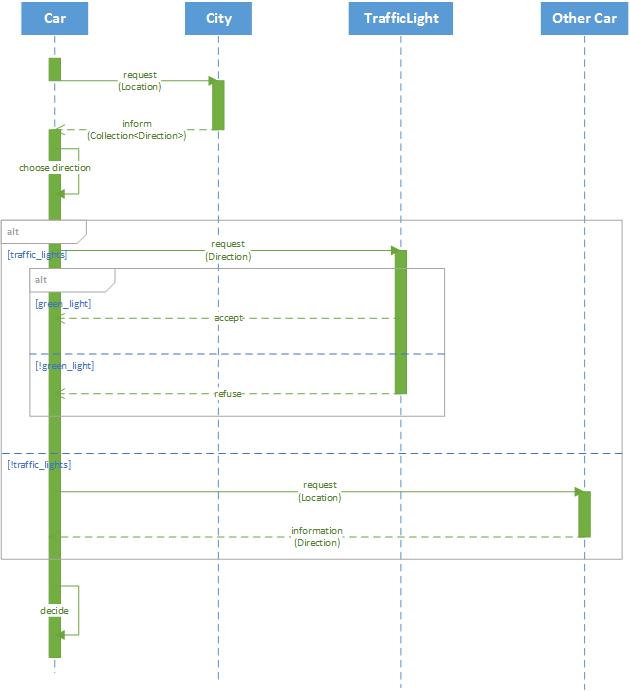
\includegraphics[width=.9\textwidth]{protocol.png}
    \caption{Schemat protokołu komunikacyjnego.}
    \label{fig:protocol}
\end{figure}

Rysunek \ref{fig:protocol} przedstawia protokół komunikacyjny przedstawiony na planie diagramu sekwencji UML. Przedstawia on sposób komunikacji \verb+Samochodu+ z~pozostałymi agentami w systemie. Komunikacja odbywa się według następującego scenariusza:

\begin{enumerate}
    \item \verb+Samochód+ nie zna dokładnej topologii ulic w~mieście. Przed dojazdem do skrzyżowania wysyła żądanie (\emph{request}) do \verb+Miasta+, podając własne położenie i~oczekując na zwrócenie listy kierunków, w~których może się poruszać.
    \item \verb+Miasto+ informuje \verb+Samochód+ o~możliwych kierunkach kontynuowania jazdy. 
    \item \verb+Samochód+, po wybraniu kierunku, sprawdza czy na skrzyżowaniu znajduje się sygnalizator. Sprawdzenie to jest możliwe dzięki wykorzystaniu domyślnego agenta \verb+Directory Facilitator+, który nie jest widoczny na schemacie.
    \item Jeżeli na skrzyżowaniu znajduje się \verb+Sygnalizator+, \verb+Samochód+ przekazuje żądanie przejechania przez skrzyżowanie, specyfikując kierunek, z~którego nadjeżdża. \verb+Sygnalizator+ wyraża zgodę (\emph{accept}) lub odrzuca żądanie (\emph{refuse}), w~zależności od obecnego stanu. 
    \item Jeżeli na skrzyżowaniu nie ma sygnalizacji świetlnej, \verb+Samochód+ żąda od innych pojazdów podania swojej pozycji. W~odpowiedzi otrzymuje informację (\emph{information}) zawierającą położenie tych pojazdów.
\end{enumerate}

Na podstawie otrzymanych informacji \verb+Samochód+ decyduje, czy może wjechać na skrzyżowanie, czy powinien się przed nim zatrzymać.

\section{Ontologia}

Tabela \ref{fig:ontology} przedstawia definicję ontologii, która będzie wykorzystywana do reprezentowania wiedzy w~obrębie systemu.

\begin{table}[ht]
    \centering
        \begin{tabular}{|c|c|c|c|c|}
            \hline
            \textbf{Koncepcja} & \textbf{Akcja} & \multicolumn{3}{c|}{\textbf{Predykat}} \\
            \hline
            & & \textbf{Nazwa} & \textbf{Typ} & \textbf{Wymagalność} \\
            \hline
            \multirow{6}{*}{Samochód} & & Pozycja X & Int & Tak \\
            \cline{3-5}
             & & Pozycja Y & Int & Tak \\
            \cline{3-5}
             & & Kierunek & Int & Tak \\
            \cline{3-5}
             & & Stan & Int & Tak \\
            \cline{2-5}
             & \multirow{2}{*}{Jazda} & Przesunięcie X & Int & Nie \\
            \cline{3-5}
             & & Przesunięcie Y & Int & Nie \\
            \hline
            \multirow{6}{*}{Sygnalizator} & & Stan & Int & Tak \\
            \cline{3-5}
             & & Pozycja X & Int & Tak \\
            \cline{3-5}
             & & Pozycja Y & Int & Tak \\
            \cline{3-5}
             & & Identyfikator & \multirow{2}{*}{Str} & \multirow{2}{*}{Tak} \\
             & & skrzyżowania & & \\
            \cline{2-5}
             & Zmiana & Nowy stan & Int & Tak \\
            \hline
            \multirow{3}{*}{Miasto} & & Rozmiar & Int & Tak \\
            \cline{3-5}
            & & Identyfikatory & \multirow{2}{*}{CEL} & \multirow{2}{*}{Tak} \\
            & & skrzyżowań & & \\
            \hline
            \multirow{3}{*}{Skrzyżowanie} & & Pozycja X & Int & Tak \\
            \cline{3-5}
             & & Pozycja Y & Int & Tak \\
            \cline{3-5}
             & & Kierunki & CEL & Tak \\
            \hline
            \multirow{5}{*}{Mapa} & & Wysokość & Int & Tak \\
            \cline{3-5}
             & & Szerokość & Int & Tak \\
            \cline{2-5}
            & \multirow{3}{*}{Wyświetlanie} & Częstotliwość & \multirow{3}{*}{Int} & \multirow{3}{*}{Nie} \\
            & & aktualizacji & & \\
            & & danych & & \\
            \hline
        \end{tabular}

        \caption{Słownik ontologii.}
        \label{fig:ontology}
\end{table}

\end{document}
